\documentclass{report}

\usepackage{lipsum}
\usepackage[margin=1in,left=1.2in,includefoot]{geometry}

\usepackage{graphicx}
\usepackage{float}

\usepackage[hidelinks]{hyperref}

% header and foot stuff
\usepackage{fancyhdr}
\pagestyle{fancy}
\fancyhead{}
\fancyfoot{}
\fancyfoot[R]{\thepage}
\renewcommand{\headrulewidth}{0pt}
\renewcommand{\footrulewidth}{0.5pt}

\begin{document}

\begin{titlepage}

	\begin{center}
	
	\line(1,0){300}\\
	[0.25cm]
	\huge{\bfseries Title}\\
	[0.25cm]
	\line(1,0){300}\\
	[10cm]

	\end{center}

	\begin{flushright}
	
	\textsc{\large{addsdsd}}\\	
	
	\end{flushright}


\end{titlepage}

\pagenumbering{roman}

\section*{Summary}
\addcontentsline{toc}{section}{\numberline{}Summary}
this is summary
\cleardoublepage

\section*{Acknoledge}
\addcontentsline{toc}{section}{\numberline{}Acknoledge}
this is Acknoledge
\cleardoublepage

\tableofcontents
\thispagestyle{empty}
\cleardoublepage


\listoffigures
\addcontentsline{toc}{section}{\numberline{}List of Figures}
\cleardoublepage

\listoftables
\addcontentsline{toc}{section}{\numberline{}List of Tables}
\cleardoublepage


\setcounter{page}{1}

\pagenumbering{arabic}

\section{Introduction}\label{sec:intro}

\lipsum[1]\

\lipsum[2]\

\lipsum[3]\

\lipsum[4]\

\lipsum[5]\

\lipsum[6]\

\lipsum[7]\

\section{Methodology}\label{sec:meth}
\subsection{materials}

\subsubsection{sources}

\lipsum[8]\
\lipsum[9]\

Figure \ref{fig:gland30} shows land use\\

\lipsum[9]\

Figure \ref{fig:gland30_2} shows land use\\

\lipsum[10]\
\lipsum[11]\

the intro is found on page \pageref{sec:intro}


\begin{figure}
	\centering
	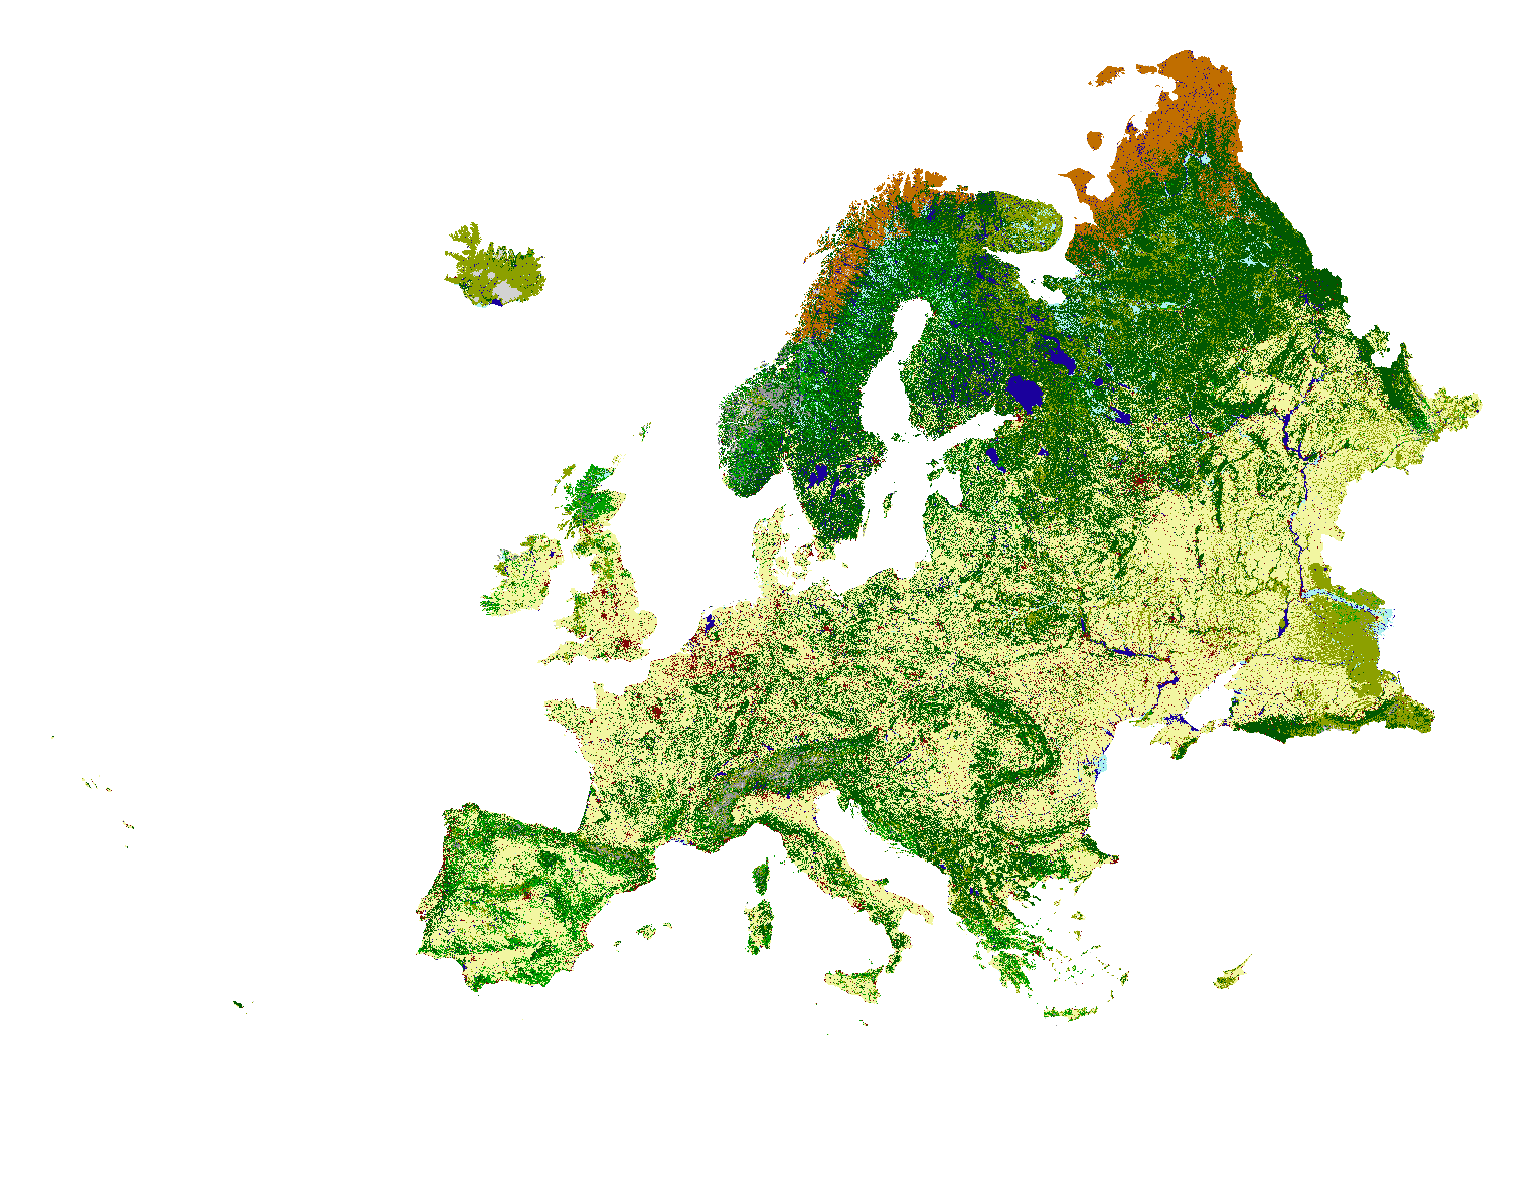
\includegraphics[scale=0.5]{/home/fcfahl/Documents/01_Latex/Test/GLand30.png}
	\caption[Option caption]{GLand30}
	\label{fig:gland30}
\end{figure}


\lipsum[10]\

\lipsum[11]\

\lipsum[10]\

\begin{figure}
	\centering
	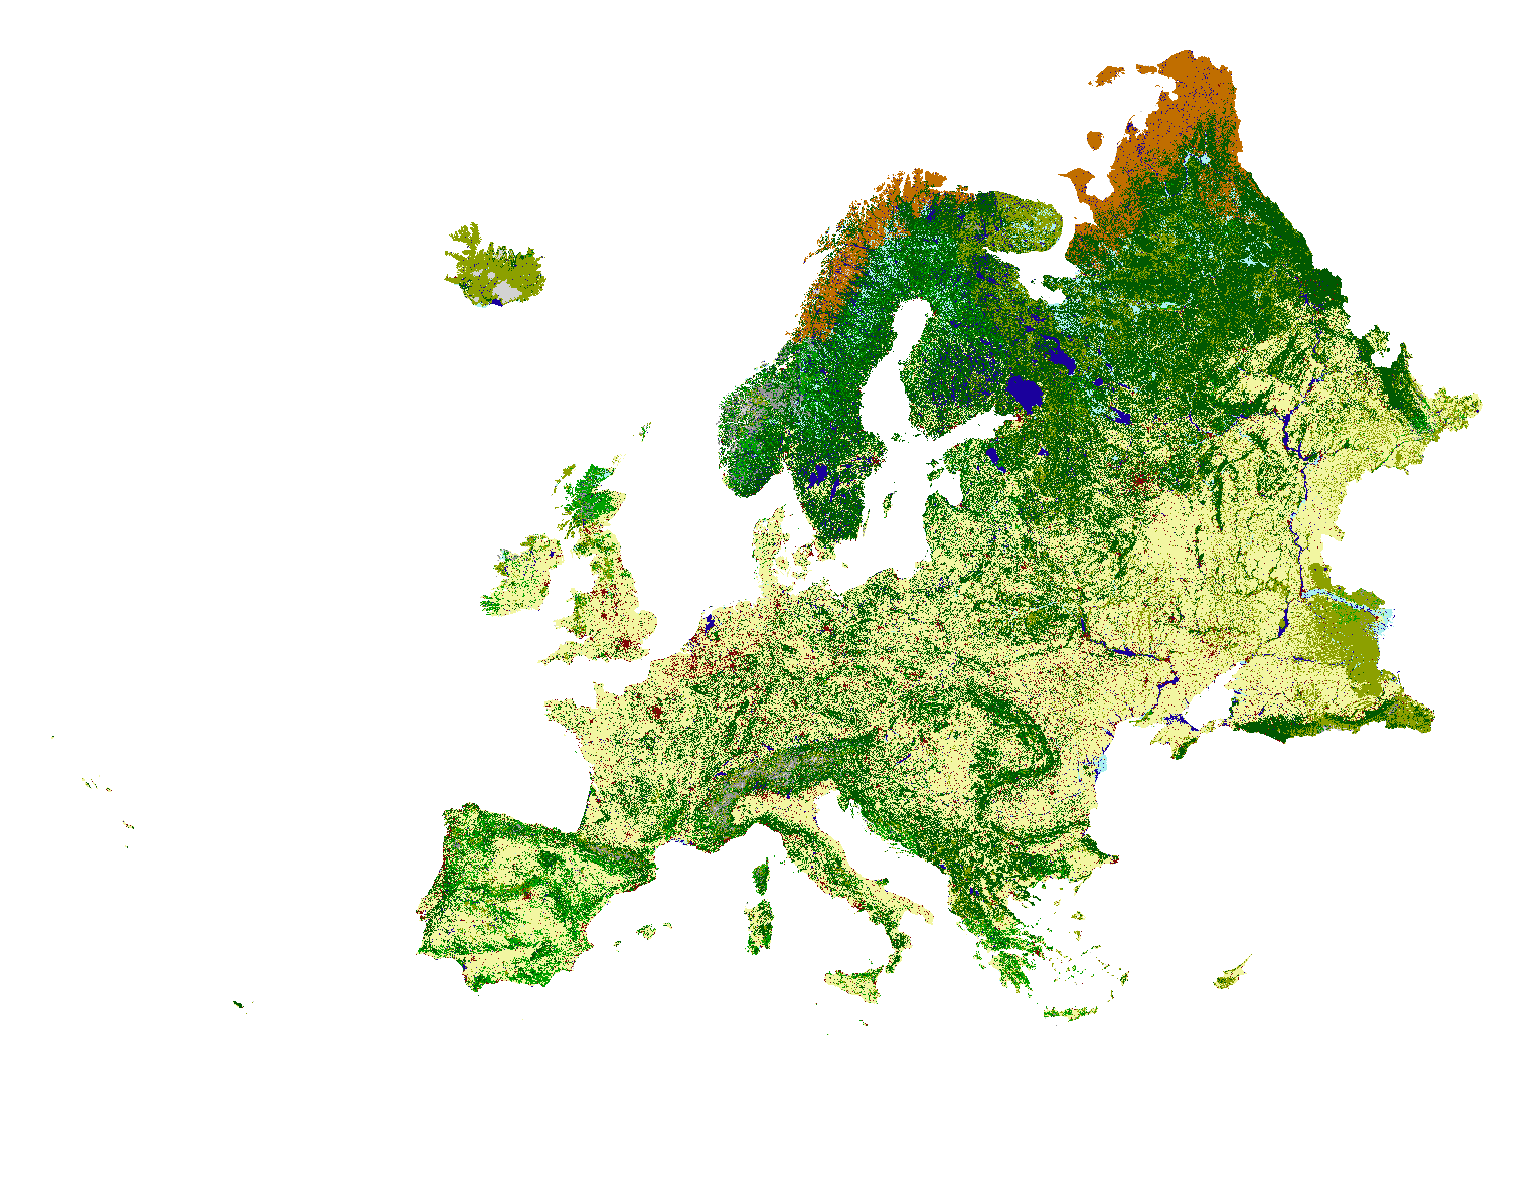
\includegraphics[scale=0.5]{/home/fcfahl/Documents/01_Latex/Test/GLand30.png}
	\caption[Option caption]{GLand30}
	\label{fig:gland30_2}
\end{figure}

\lipsum[11]\

Table \ref{tab:test table 1} sjhows.....

\lipsum[10]\

\lipsum[11]\

\begin{table}[H]

	\centering
	\caption[this is an optional caption, without reference]{local caption, with reference}
	\label{tab:test table 1}
	\begin{tabular}{lcr}
		\bfseries{col1} & col2 & col3\\
		1 & a & q\\
		2 & b & a\\
		3 & c & s\\		
		4 & d & d\\
		5 & e & c\\		
		
	
	\end{tabular}

\end{table}

\lipsum[10]\

\lipsum[11]\

\begin{table}[H]

	\centering
	\caption{import table}
	\label{tab:xls table}
	\begin{tabular}{p{0.9in}p{0.9in}p{0.9in}}
		Theme & Topic1 & Topic2\\
		M1 & MODIS & LULC\\

		
	
	\end{tabular}

\end{table}


\end{document}